\subsection{Adding Perpendicular to Chains}

In the upper left quadrant: Period adding perpendicular to the direction of chains.
Chains also not connected.

Cycle at point $A_8$: $\Cycle{\L^4\R^4}$, at point $C_{10}$: $\Cycle{\L^5\R^5}$.
The parameter regions overlap and both cycles exist at point $B_{8, 10}$.

The chain of period 9 is not connected.
The cycle at point $A_9$ is $\Cycle{\L^5\R^4}$ and at point $C_9$ its $\Cycle{\L^4\R^5}$.
The parameter regions do not overlap with each other.

\begin{figure}
    \centering
    \begin{subfigure}{0.4\textwidth}
        \centering
        \includegraphics[width=\textwidth]{70_030_SearchAdding_quad2/2D_Period_UpperLeft/result.png}
        \caption{Full}
        %        \label{fig:final.period.whole.full}
    \end{subfigure}
    \begin{subfigure}{0.4\textwidth}
        \centering
        \includegraphics[width=\textwidth]{70_030_SearchAdding_quad2/2D_Period_UpperLeft_Zoomed/result.png}
        \caption{Zoomed-In}
        %        \label{fig:final.period.whole.halved}
    \end{subfigure}
    \caption{2D Scans of Periods of Upper Left Quarter Of Quad2 Model}
\end{figure}

\begin{figure}
    \centering
    \includegraphics[width=0.6 \textwidth]{70_030_SearchAdding_quad2/2D_Regions_UpperLeft_Zoomed/result.png}
    %        \label{fig:final.period.whole.halved}
    \caption{2D Scans of Period Regions in Upper Left Quarter Of Quad2 Model}
\end{figure}

\begin{figure}
    \centering
    \begin{subfigure}{0.4\textwidth}
        \centering
        \includegraphics[width=\textwidth]{70_030_SearchAdding_quad2/1D_Period_UpperLeft_B8_C9/result.png}
        \caption{Between $B_8$ and $C_9$}
        %        \label{fig:final.period.whole.full}
    \end{subfigure}
    \begin{subfigure}{0.4\textwidth}
        \centering
        \includegraphics[width=\textwidth]{70_030_SearchAdding_quad2/1D_Period_UpperLeft_C10_C9/result.png}
        \caption{Between $C_{10}$ and $C_9$}
        %        \label{fig:final.period.whole.halved}
    \end{subfigure}
    \caption{1D Scans of Periods of Upper Left Quarter Of Quad2 Model}
\end{figure}

\begin{figure}
    \centering
    \begin{subfigure}{0.3\textwidth}
        \centering
        \includegraphics[width=\textwidth]{70_030_SearchAdding_quad2/Cobweb_UpperLeft_A8/result.png}
        \caption{At $A_{8}$}
        %        \label{fig:final.period.whole.full}
    \end{subfigure}
    \begin{subfigure}{0.3\textwidth}
        \centering
        \includegraphics[width=\textwidth]{70_030_SearchAdding_quad2/Cobweb_UpperLeft_B810/result.png}
        \caption{At $B_{8, 10}$}
        %        \label{fig:final.period.whole.full}
    \end{subfigure}
    \begin{subfigure}{0.3\textwidth}
        \centering
        \includegraphics[width=\textwidth]{70_030_SearchAdding_quad2/Cobweb_UpperLeft_C10/result.png}
        \caption{At $C_{10}$}
        %        \label{fig:final.period.whole.halved}
    \end{subfigure}
    \caption{Cobwebs at Selected Points of Upper Left Quarter Of Quad2 Model}
\end{figure}